\documentclass[12pt,twoside]{article}
%%%%%%%%%%%%%%%%%%%%%%%%%%%%%%%%%%%%%%%%%%%%%%%%%%%%%%%%%%%%%
% Meta informations:
\newcommand{\trauthor}{Daniel Speck}
\newcommand{\trtype}{Seminar Paper} %{Seminararbeit} %{Proseminararbeit}
\newcommand{\trcourse}{Brain Modelling}
\newcommand{\trtitle}{Deep Learning: Neural Networks for Object Detection and Tracking Tasks}
\newcommand{\trmatrikelnummer}{632 13 17}
\newcommand{\tremail}{2speck@informatik.uni-hamburg.de}
\newcommand{\trarbeitsbereich}{Knowledge Technology, WTM}
\newcommand{\trdate}{29.05.2015}

%%%%%%%%%%%%%%%%%%%%%%%%%%%%%%%%%%%%%%%%%%%%%%%%%%%%%%%%%%%%%
% Languages:

% Falls die Ausarbeitung in Deutsch erfolgt:
% \usepackage[german]{babel}
% \usepackage[T1]{fontenc}
% \usepackage[latin1]{inputenc}
% \usepackage[latin9]{inputenc}	 				
% \selectlanguage{german}

% If the thesis is written in English:
\usepackage[english]{babel} 						
\selectlanguage{english}

%%%%%%%%%%%%%%%%%%%%%%%%%%%%%%%%%%%%%%%%%%%%%%%%%%%%%%%%%%%%%
% Bind packages:
\usepackage{acronym}                    % Acronyms
\usepackage{algorithmic}								% Algorithms and Pseudocode
\usepackage{algorithm}									% Algorithms and Pseudocode
\usepackage{amsfonts}                   % AMS Math Packet (Fonts)
\usepackage{amsmath}                    % AMS Math Packet
\usepackage{amssymb}                    % Additional mathematical symbols
\usepackage{amsthm}
\usepackage{booktabs}                   % Nicer tables
%\usepackage[font=small,labelfont=bf]{caption} % Numbered captions for figures
\usepackage{color}                      % Enables defining of colors via \definecolor
\definecolor{uhhRed}{RGB}{254,0,0}		  % Official Uni Hamburg Red
\definecolor{uhhGrey}{RGB}{122,122,120} % Official Uni Hamburg Grey
\usepackage{fancybox}                   % Gleichungen einrahmen
\usepackage{fancyhdr}										% Packet for nicer headers
%\usepackage{fancyheadings}             % Nicer numbering of headlines

%\usepackage[outer=3.35cm]{geometry} 	  % Type area (size, margins...) !!!Release version
%\usepackage[outer=2.5cm]{geometry} 		% Type area (size, margins...) !!!Print version
%\usepackage{geometry} 									% Type area (size, margins...) !!!Proofread version
\usepackage[outer=3.15cm]{geometry} 	  % Type area (size, margins...) !!!Draft version
\geometry{a4paper,body={5.8in,9in}}

\usepackage{graphicx}                   % Inclusion of graphics
%\usepackage{latexsym}                  % Special symbols
\usepackage{longtable}									% Allow tables over several parges
\usepackage{listings}                   % Nicer source code listings
\usepackage{multicol}										% Content of a table over several columns
\usepackage{multirow}										% Content of a table over several rows
\usepackage{rotating}										% Alows to rotate text and objects
\usepackage[hang]{subfigure}            % Allows to use multiple (partial) figures in a fig
%\usepackage[font=footnotesize,labelfont=rm]{subfig}	% Pictures in a floating environment
\usepackage{tabularx}										% Tables with fixed width but variable rows
\usepackage{url,xspace,boxedminipage}   % Accurate display of URLs

%%%%%%%%%%%%%%%%%%%%%%%%%%%%%%%%%%%%%%%%%%%%%%%%%%%%%%%%%%%%%
% Configurationen:

\hyphenation{whe-ther} 									% Manually use: "\-" in a word: Staats\-ver\-trag

%\lstloadlanguages{C}                   % Set the default language for listings
\DeclareGraphicsExtensions{.pdf,.svg,.jpg,.png,.eps} % first try pdf, then eps, png and jpg
\graphicspath{{./src/}} 								% Path to a folder where all pictures are located
\pagestyle{fancy} 											% Use nicer header and footer

% Redefine the environments for floating objects:
\setcounter{topnumber}{3}
\setcounter{bottomnumber}{2}
\setcounter{totalnumber}{4}
\renewcommand{\topfraction}{0.9} 			  %Standard: 0.7
\renewcommand{\bottomfraction}{0.5}		  %Standard: 0.3
\renewcommand{\textfraction}{0.1}		  	%Standard: 0.2
\renewcommand{\floatpagefraction}{0.8} 	%Standard: 0.5

% Tables with a nicer padding:
\renewcommand{\arraystretch}{1.2}

%%%%%%%%%%%%%%%%%%%%%%%%%%%%
% Additional 'theorem' and 'definition' blocks:
\theoremstyle{plain}
\newtheorem{theorem}{Theorem}[section]
%\newtheorem{theorem}{Satz}[section]		% Wenn in Deutsch geschrieben wird.
\newtheorem{axiom}{Axiom}[section] 	
%\newtheorem{axiom}{Fakt}[chapter]			% Wenn in Deutsch geschrieben wird.
%Usage:%\begin{axiom}[optional description]%Main part%\end{fakt}

\theoremstyle{definition}
\newtheorem{definition}{Definition}[section]

%Additional types of axioms:
\newtheorem{lemma}[axiom]{Lemma}
\newtheorem{observation}[axiom]{Observation}

%Additional types of definitions:
\theoremstyle{remark}
%\newtheorem{remark}[definition]{Bemerkung} % Wenn in Deutsch geschrieben wird.
\newtheorem{remark}[definition]{Remark} 

%%%%%%%%%%%%%%%%%%%%%%%%%%%%
% Provides TODOs within the margin:
\newcommand{\TODO}[1]{\marginpar{\emph{\small{{\bf TODO: } #1}}}}

%%%%%%%%%%%%%%%%%%%%%%%%%%%%
% Abbreviations and mathematical symbols
\newcommand{\modd}{\text{ mod }}
\newcommand{\RS}{\mathbb{R}}
\newcommand{\NS}{\mathbb{N}}
\newcommand{\ZS}{\mathbb{Z}}
\newcommand{\dnormal}{\mathit{N}}
\newcommand{\duniform}{\mathit{U}}

\newcommand{\erdos}{Erd\H{o}s}
\newcommand{\renyi}{-R\'{e}nyi}
%%%%%%%%%%%%%%%%%%%%%%%%%%%%%%%%%%%%%%%%%%%%%%%%%%%%%%%%%%%%%
% Document:
\begin{document}
\renewcommand{\headheight}{14.5pt}

\fancyhead{}
\fancyhead[LE]{ \slshape \trauthor}
\fancyhead[LO]{}
\fancyhead[RE]{}
\fancyhead[RO]{ \slshape \trtitle}

%%%%%%%%%%%%%%%%%%%%%%%%%%%%
% Cover Header:
\begin{titlepage}
	\begin{flushleft}
		Universit\"at Hamburg\\
		Department Informatik\\
		\trarbeitsbereich\\
	\end{flushleft}
	\vspace{3.5cm}
	\begin{center}
		\huge \trtitle\\
	\end{center}
	\vspace{3.5cm}
	\begin{center}
		\normalsize\trtype\\
		[0.2cm]
		\Large\trcourse\\
		[1.5cm]
		\Large \trauthor\\
		[0.2cm]
		\normalsize Matr.Nr. \trmatrikelnummer\\
		[0.2cm]
		\normalsize\tremail\\
		[1.5cm]
		\Large \trdate
	\end{center}
	\vfill
\end{titlepage}

	%backsite of cover sheet is empty!
\thispagestyle{empty}
\hspace{1cm}
\newpage

%%%%%%%%%%%%%%%%%%%%%%%%%%%%
% Abstract:

% Abstract gives a brief summary of the main points of a paper:
\section*{Abstract}
Deep neural networks are one of the most successful learning strategies at the moment as the computing power for creating such structures rised in the past years via GPU computing. Object detection and tracking tasks can be fulfilled with these architectures.
  

% Lists:
\setcounter{tocdepth}{2} 					% depth of the table of contents (for Seminars 2 is recommented)
\tableofcontents
\pagenumbering{arabic}
\clearpage






%%%%%%%%%%%%%%%%%%%%%%%%%%%%
% Content:

% the actual content, usually separated over a number of sections
% each section is assigned a label, in order to be able to put a
% crossreference to it




\section{Introduction}
\label{sec:introduction}

Deep learning is subcategory of machine learning and the focus of this paper will be deep neural networks in the context of deep learning.
\\
An overview of image classification will be made \cite{MultiColumnDeepNeuralNetworksClassification-Ciresan} \cite{ImangeNetClassificationCNN-Krizhevsky}.
\\
The visual cortex and deep learning strategies will be introduced \cite{DeepHierarchiesVisualCortex-kruger}.
\\
Approaches for object detection \cite{DeepNeuralNetworksObjectDetection-Szegedy} and tracking \cite{LearningDeepCompactImageTracking-Wang} via deep neural networks will be discussed.




\section{Background information: Artificial neural networks}
\label{sec:ann}

Briefly introduction for classic artificial neural networks without GPU computing.




\section{Deep neural networks}
\label{sec:dnn}

Overview for classic deep neural networks. Details about different concepts and approaches.




\section{Convolutional neural networks and image processing}
\label{sec:cnn}

For deep learning purposes (classic / fully-connected) multilayer perceptrons consume a sizable amount of resources for proper training when they are designed to solve complex tasks because the amount of neurons and especially weights increases rapidly with the network's size.
\\
For example, a MLP with three layers, an input layer with 100 neurons, a hidden layer with 25 neurons and an output layer with 10 neurons for classifying images with a size of 10x10 pixels into 10 different classes would have $100 * 25 + 25 * 10 = 2,750$ weights/connections. Training this net would already result in a big time and space complexity. Moreover, as features in images capturing real world scenes are distributed in certain patterns (they cover spatially local correlation, such as shapes), there is no need to have every pixels information being processed by one neuron. Actually in most cases results would be even better, if the pixels information is pre-processed, for instance by edge detection filters but a fully connected layer of neurons is not an optimal solution for this task.
\\
Convolutional neural networks (CNNs) are inspired by biology, instead of connecting every pixels information directly with a neuron to process its information it filters the information in the first layers \cite{ImangeNetClassificationCNN-Krizhevsky}. This procedure is similar to the on processes happening when an biological eye receives stimuli.
\\
The receptive field \footnote{\url{http://en.wikipedia.org/wiki/Receptive_field}} has a vast amount of photoreceptor cells \footnote{\url{http://en.wikipedia.org/wiki/Photoreceptor_cell}} gathering information and converging the received information on to distinctly less retinal ganglion cells \footnote{\url{http://en.wikipedia.org/wiki/Retinal_ganglion_cell}}. This process maps several features and reduces the input dimensionality as well as distinguishes the information to separate "channels" which are then transfered to the corresponding neurons to process features such as color, motion, shapes and so on separately \cite{DeepHierarchiesVisualCortex-kruger}.
\\
The idea of CNNs is based on this biological processes, the information of an input image is convolved by several filters which try to extract interesting features in the first layer and in following layers this information is pooled and subsampled \cite{ImangeNetClassificationCNN-Krizhevsky}.
\\
Convolution itself is the applying of a function repeatedly of the output of another function and in the context of CNNs it is applying different "filters" over an image to extract the already mentioned features. A convolution layer extracts the pixel information out of an image with kernels \footnote{\url{http://en.wikipedia.org/wiki/Kernel_(image_processing)}}.
\\
\\
Example for a convolution layer: In figure \ref{fig:animal-edge-detection} you can see an image of an animal on the left side (original image) and a kernel processed one on the right side. The used kernel matrix was:
\begin{equation}
	\label{equation:kernal-matrix}
	\begin{bmatrix}
	-1 & -1 & -1 \\
	-1 & 8 & -1 \\
	-1 & -1 & -1 \\
	\end{bmatrix}
\end{equation}
So basically each pixels information in the right, processed image is the result of applying the kernel matrix (\ref{equation:kernal-matrix}) on the same pixel (and the neighboring pixels) in the left image.

\begin{figure}
  	\centerline{
  		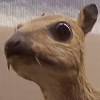
\includegraphics[width=0.3\textwidth]{animal-original.png}
  		\qquad
  		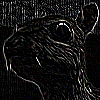
\includegraphics[width=0.3\textwidth]{animal-edge-detection.png}
  		}
 	{\caption{Left side: original image, right side: edge-detection kernel processed image. Original image by Michael Plotke, 28th of January, 2013. Open creative commons license.
 	\protect\url{http://upload.wikimedia.org/wikipedia/commons/5/50/Vd-Orig.png} and \protect\url{http://upload.wikimedia.org/wikipedia/commons/6/6d/Vd-Edge3.png}}\label{fig:animal-edge-detection}}
 \end{figure}



\section{Research and field of application}
\label{sec:research_and_application}


\subsection{Image classification}
More details / information about state of the art object/image detection/classification.


\subsection{Video classification}
More details / information about state of the art object/video detection/classification.


\subsection{Object tracking}



\section{Conclusion}
\label{sec:concl}

Conclusion of the paper.




%%%%%%%%%%%%%%%%%%%%%%%%%%%%%%%%%%%%%%
% hier werden - zum Ende des Textes - die bibliographischen Referenzen
% eingebunden
%
% Insbesondere stehen die eigentlichen Informationen in der Datei
% ``bib.bib''
%
\newpage
\bibliographystyle{plain}
\addcontentsline{toc}{section}{Bibliography}% Add to the TOC
\bibliography{bib}


\end{document}


